\section{Theorie}
\label{sec:Theorie}

Werden in ein Kristalgitter aus einfach positiv geladenen Kationen und einfach negativ geladenen Anionen doppelt positiv geladene Kationen eingeführt, so bilden sich zwischen diesen und im Gitter vorkommenden Fehlstellen Dipolmomente aus. Dies beruht darauf, dass sich im Ursprungsgitter die Ladungen der Anionen und Kationen lokal aufheben und einen global neutralen Kristall ergeben. Das Fehlen eines Kations führt somit zu einer lokalen negativen Ladung, während die doppelt geladenen Kationen zu einem lokalen Überschuss positiver Ladung führen. Dies ist in Abb. \ref{fig:fehlstelle} schematisch dargestellt.

\begin{figure}
  \centering
  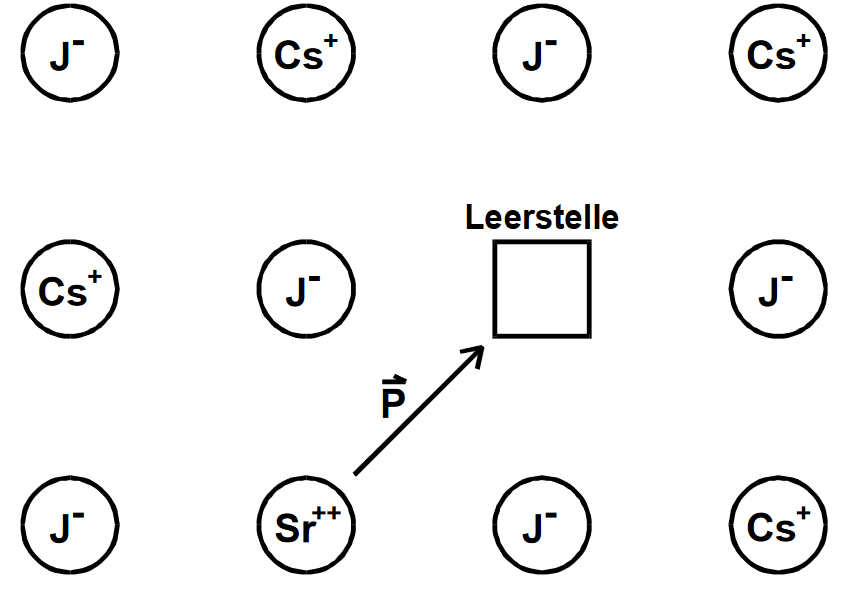
\includegraphics{./logos/Fehlstelle.PNG}
  \caption{Schematische Darstellung der Entstehung von Dipolmomenten in Kristallgittern.\cite{Anleitung}}
  \label{fig:fehlstelle}
\end{figure}

Da auf diese Weise erzeugte Dipolmomente an die Symmetrie des Gitters gebunden sind, welches sie hervorruft, sind nur diskrete Orientierungen und Beträge möglich, welche statistisch verteilt sind. Durch thermisch bedingte Bewegung der Gitterionen, können Fehlstellen durch den Kristall wandern, was es den Dipolmomenten ermöglicht, ihre Orientierung zu ändern. Um die Orientierung zu ändern, muss die Aktivierungsenergie $W$ aufgebracht werden, um eine Leerstelle im durch das Kristallgitter hervorgerufenen Potential diffundieren zu lassen. Da $W$ durch thermische Energie aufgebracht werden muss, genügt die energetische Verteilung der Dipole der Boltzmann-Statistik.
Diese beiden Faktoren führen dazu, dass durch ein äußeres $E$-Feld ausgelenkte Dipole $\vec{p}$ nach einer mittleren, Temperatur $T$ abhängigen, Zeit
\begin{equation}
  \tau (T) = \tau_0 \exp{\left(\frac{W}{kT}\right)}
  \label{eqn:relaxation}
\end{equation}
in eine statistische Verteilung über gehen. $\tau_0$ bezeichnet hierbei die sogenannte charakteristische Relaxationszeit. Es lässt sich unter der Bedingung, dass $pE<<kT$ gilt, allerdings nur ein Anteil von
\begin{equation}
    y(T) = \frac{pE}{3kT}
\end{equation}
Dipolen in Richtung des Feldes auslenken.
Da $\tau$ gemäß \eqref{eqn:relaxation} temperaturabhängig ist, lassen sich Dipole durch zügiges abkühlen "einfrieren". Heizt man anschließend den zu untersuchenden Kristall mit konstanter Heizrate
\begin{equation}
  H := \frac{\symup{d}T}{\symup{d}t} = \text{const}
  \label{eqn:heizrate}
\end{equation}
auf, so fließt durch die Relaxation der Dipole eine Relaxationsstromdichte $j$ von
\begin{equation}
  j(T) = y(T_p) \cdot p \cdot\frac{\symup{d}N}{\symup{d}t}.
  \label{eqn:dichteansatz}
\end{equation}
Hierbei bezeichnet $\frac{\symup{d}N}{\symup{d}t}$ die Rate, mit der die Dipole relaxieren, und $y(T_p)$ den Anteil der vor der Abkühlung ausgerichteten Dipole.
Da die Relaxationsrate der Dipole mit Relaxationszeit $\tau(T)$ wie bei radioaktiven Zerfällen proportional zur Anzahl $N$ an noch ausgerichteten Dipolen ist, erhält man über
\begin{equation}
  \frac{\symup{d}N}{\symup{d}t} = -\frac{N}{\tau(T)}
  \label{eqn:dN}
\end{equation}
einen Ausdruck für $N(t)$, welcher sich mittels \eqref{eqn:heizrate} zu
\begin{equation}
  N(T) = N_p \exp{-\frac{1}{H}\int^T_{T_0} \frac{\symup{d}T'}{\tau(T')}}
  \label{eqn:N}
\end{equation}
umschreiben lässt.
Als endgültiger Ausdruck für $j(T)$ findet sich dann
\begin{equation}
  j(T) = \frac{p^2E}{3kT_p}\frac{N_p}{\tau_0}\exp{\left(-\frac{1}{H}\int^T_{T_0}\exp{\left(-\frac{W}{kT'}\right)}\symup{d}T'\right)}\exp{\left(-\frac{W}{kT}\right)}.
  \label{eqn:jKomplett}
\end{equation}

Durch Näherung des Integrals wird dieser Ausdruck zu Beginn der Stromkurve \ref{fig:strom-theo}, welche sich über $i(T)=Fj(T)$ mit $F$ als Querschnittsfläche der Probe bestimmen lässt, hinreichend durch
\begin{equation}
  j(T) \approx \frac{p^2 E N_p}{3kT_p\tau_0}\exp{\left(\frac{-W}{kT}\right)}
  \label{eqn:dichtefertig}
\end{equation}
beschrieben.

\begin{figure}
  \centering
  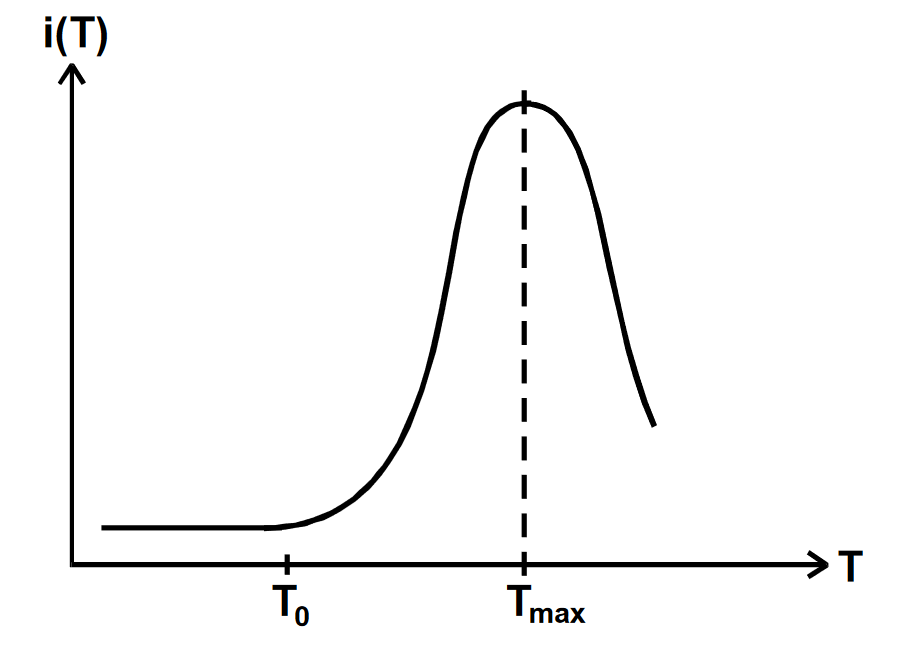
\includegraphics{./logos/Strom_theorie.PNG}
  \caption{Erwarteter qualitativer Verlauf des Depolarisationsstromes $i(t)$ \cite{Anleitung}.}
  \label{fig:strom-theo}
\end{figure}

Der das Maximum des Stromverlaufs rührt daher, dass der Strom durch den Abfall von $\tau(T)$ mit steigender Temperatur zunächst zunimmt, allerdings fällt die Relaxationsrate stetig gemäß \eqref{eqn:dN}. Es kann ein zweites Maximum auftreten, welches durch weitere Relaxationen mit höherem $W$ hervorgerufen wird.
Ohne das Integral zu nähern lässt sich $\tau(T)$ durch Integration des Stromes nach
\begin{equation}
  \tau(T) = \frac{\int_{T}^{\infty}i(T')\symup{d}T'}{bi(T)}
  \label{eqn:tau2}
\end{equation}
berechnen.
Aus einem gemessenen Verlauf $i(T)$ lässt sich somit $W$ durch die Steigung einer linearen Ausgleichsgeraden an die logarithmierten Verläufe von \eqref{eqn:tau2}, bzw. \eqref{eqn:dichtefertig}, bestimmen.
Zur Bestimmung von $\tau_0$ betrachtet man die Lage des Maximums von $i(T)$. Dieses liegt nach \eqref{eqn:jKomplett} bei
\begin{equation}
  \tau_{max}(T) = \frac{kT_{max}^2}{HW}.
  \label{eqn:tau3}
\end{equation}
Mit Hilfe dieses Wertes und \eqref{eqn:relaxation} lässt sich nun $\tau_0$ berechnen.
